\section{Experiments}
\label{sec:05_exp}

\subsection{Datasets}
\label{subsec:subsec_51_datasets}
We evaluate BiDecT on three standard video captioning benchmarks: MSVD~\cite{chenCollectingHighlyParallel2011}, MSR-VTT~\cite{xuMSRVTTLargeVideo2016}, and VATEX~\cite{wangVaTeXLargeScaleHighQuality2019}.

\textbf{MSVD} contains 1,970 short video clips with an average duration of approximately 10 seconds, each annotated with around 40 captions. We follow the conventional split of 1,200/100/670 videos for training, validation, and testing, as adopted in prior work.

\textbf{MSR-VTT} is an open-domain benchmark consisting of 10,000 video clips spanning 20 categories, each paired with 20 human-annotated captions and averaging approximately 15 seconds. We adopt the standard 6,513/497/2,990 split used in prior work.

\textbf{VATEX} is a multilingual dataset containing 41,269 video clips of approximately 10 seconds each, annotated with 10 English and 10 Chinese captions. We use only the English captions and evaluate on the public test split. Because a subset of the original videos is no longer publicly accessible, the accessible subset used in our experiments contains 25,985 training, 3,000 validation, and 5,808 test videos, compared to the official split of 25,991/3,000/6,000.

% ==== TODO: Reasons for choosing 3 datasets ====
% Together, these three benchmarks span a wide range of scales (from approximately 2,000 videos in MSVD to over 41,000 in VATEX) and annotation densities (from 10 to 40 captions per video), enabling evaluation across both low-resource and large-scale settings. Their widespread adoption in recent literature also facilitates direct comparison with recent state-of-the-art methods.


\subsection{Evaluation Metrics}
\label{subsec:subsec_52_metrics}

% ========== Detail version ==========
% We evaluate BiDecT using four standard automatic metrics for video captioning: BLEU@4 (B4)~\cite{papineniBleuMethodAutomatic2002}, METEOR (M)~\cite{banerjeeMETEORAutomaticMetric2005}, ROUGE-L (R)~\cite{linAutomaticEvaluationMachine2004}, and CIDEr (C)~\cite{vedantamCIDErConsensusbasedImage2015}.

% \textbf{BLEU@4} measures modified $n$-gram precision between a generated caption and its references using $n$-gram matches up to order 4:
% \begin{equation}
% \mathrm{BLEU@N}=\mathrm{BP}\cdot\exp{\left(\sum_{n=1}^{N}w_n\mathrm{\;log\;} p_n\right)},
% \end{equation}
% where $p_n$ denotes the clipped $n$-gram precision, $w_n=1/N$ are uniform weights, and BP is the brevity penalty discouraging overly short outputs. BLEU primarily reflects local lexical precision and is sensitive to exact word matches.

% \textbf{METEOR} computes a recall-oriented alignment score that additionally considers stemming and synonym matching, making it more sensitive to semantic similarity than BLEU.
% \begin{equation}
% \mathrm{METEOR}=F_\alpha\cdot\left(1-\gamma\cdot f^\beta\right),
% \end{equation}
% where $F_\alpha=\frac{P\cdot R}{\alpha P+(1-\alpha)R}$ and $f$ is the ratio of contiguous matching chunks to total matched unigrams. Matching extends beyond exact tokens to include stems and synonyms.

% \textbf{ROUGE-L} evaluates sentence-level similarity based on the longest common subsequence (LCS) between generated and reference captions, capturing fluency and sequence consistency without requiring contiguous matches.
% \begin{equation}
% F_{lcs}=\frac{\left(1+\beta^2\right)\cdot R_{lcs}\cdot P_{lcs}}{R_{lcs}+\beta^2\cdot P_{lcs}},
% \end{equation}
% where $R_{lcs}=\mathrm{|LCS|}/m$ and $P_{lcs}=\mathrm{|LCS|}/n$, with $m$ and $n$ denoting the lengths of the reference and candidate sentences, respectively.

% \textbf{CIDEr} is specifically designed for captioning tasks. It represents captions as TF-IDF weighted $n$-gram vectors and computes the consensus similarity between a generated caption $c_i$ and a set of reference captions $S_i$:
% \begin{equation}
% \mathrm{CIDEr}(c_i,S_i)=\sum_{n=1}^{N}w_n\cdot{\mathrm{CIDEr}}_n(c_i,S_i),
% \end{equation}
% with
% \begin{equation}
% {\mathrm{CIDEr}}_n(c_i,S_i)=\frac{1}{M}\sum_{j=1}^{M}\frac{\mathbf{g}^n(c_i)\cdot\mathbf{g}^n(s_{ij})}{\parallel\mathbf{g}^n(c_i)\parallel\; \parallel\mathbf{g}^n(s_{ij})\parallel},
% \end{equation}
% where $\mathbf{g}^n(\cdot)$ denotes the TF-IDF weighted $n$-gram representation, $M$ is the number of reference captions, and \mbox{$w_n=1/N$} are uniform weights over different $n$-gram orders. By emphasizing informative and consensus-driven $n$-grams, CIDEr has been shown to correlate more strongly with human judgments of caption quality than other automatic metrics.

% Following established practice in video captioning research, CIDEr is adopted as the primary evaluation metric. All metrics are computed using the Microsoft COCO Caption Evaluation toolkit following the standard evaluation protocol adopted in prior video captioning literature.
% ====================================

% TODO: Short version here!!!
We evaluate BiDecT using four standard automatic metrics for video captioning: BLEU@4 (B4)~\cite{papineniBleuMethodAutomatic2002}, which measures modified $n$-gram precision and reflects local lexical accuracy; METEOR (M)~\cite{banerjeeMETEORAutomaticMetric2005}, a recall-oriented metric that additionally considers stemming and synonym matching for greater sensitivity to semantic similarity; ROUGE-L (R)~\cite{linAutomaticEvaluationMachine2004}, which evaluates sentence-level similarity based on the longest common subsequence; and CIDEr (C)~\cite{vedantamCIDErConsensusbasedImage2015}, which computes TF-IDF weighted $n$-gram consensus and has been shown to correlate strongly with human judgments of caption quality. Following established practice, CIDEr is adopted as the primary metric. All scores are computed using the Microsoft COCO Caption Evaluation toolkit.


\subsection{Implementation}
\label{subsec:subsec_53_implement}
\textbf{Video Preprocessing}. All raw videos are resized to 240 pixels on the shorter side while preserving aspect ratio and re-encoded using the H.264 codec via FFmpeg with $\mathrm{KeyInt}$ set to 45. For each video, at most $G$ GOPs are sampled, uniformly distributed over time when the total GOP count exceeds $G$. $G$ is set to the 75th percentile of the GOP-count distribution in each training set, yielding $G\,\texttt{=}\,$8, 10, and 8 for MSVD, MSR-VTT, and VATEX, respectively.

\textbf{Feature Extraction}. Following the process in Section~\ref{subsec:subsec_42_extraction}, all multimodal features are pre-extracted offline and stored in HDF5 format. Table~\ref{tab:tab02_feature_extractors} summarizes the feature extractors and output dimensions.

\begin{table}[!t]
\caption{Feature extractors, input sources, and output dimensions for each modality in BiDecT.}
\label{tab:tab02_feature_extractors}
\centering
\begin{tabular}{l l l c}
\hline\hline
\textbf{Feature} & \textbf{Model} & \textbf{Input Source} & \textbf{Dimension} \\
\hline
Appearance & BLIP-2 OPT-2.7B & I-frame & $1{,}408$ \\
Semantic & SRoBERTa-large & BLIP-2 caption & $1{,}024$ \\
Motion & MViTv2-small & 16 sampled frames & $768$ \\
\hline\hline
\end{tabular}
\end{table}



% Table 3 
% Feature extractors, input sources, and output dimensions for each modality in BiDecT. Appearance and semantic features share the same I-frame input source but are derived from different components of BLIP-2.
% Feature	Model	Input Source	Dimension
% Appearance	BLIP-2 OPT-2.7B [25] 
% I-frame	d_A=1,408
% Semantic	all-RoBERTa-large-v1 (SRoBERTa) [32]
% BLIP-2 caption	d_S=1,024
% Motion	MViTv2-small [18]
% 16 sampled frames	d_M=768

\textbf{Model Configuration}. The model dimension is set to \mbox{$d_{\textit{model}}\,\texttt{=}\,512$}, with feed-forward dimension \mbox{$d_{\textit{ff}}\,\texttt{=}\,2048$} and 4 attention heads. Both the Backward Decoder and Forward Decoder consist of 3 stacked Transformer layers ($N_{\textit{BD}}\,\texttt{=}\,N_{\textit{FD}}\,\texttt{=}\,3$). The maximum decoding length is fixed at 20 tokens for all datasets.

\textbf{Training}. The model is trained for 16 epochs with a batch size of 64 using the Adam optimizer with the AMSGrad variant. The initial learning rate is set to $1\times{10}^{-4}$, with weight decay $0.5\times{10}^{-5}$ and gradient clipping at 5.0. The learning rate is linearly warmed up over the first 3 epochs and reduced by a factor of 0.5 when the validation loss does not improve for 3 consecutive epochs. The loss-balancing coefficient is set to $\lambda\,\texttt{=}\,0.6$, with dropout rate 0.1 and label smoothing 0.15.

\textbf{Inference}. Beam search with beam size 4 is first applied to the Backward Decoder to generate the reverse caption and the corresponding backward contextual representation $\MyLVec[1]{H}$. The Forward Decoder then generates the final caption conditioned on this fixed context. The checkpoint with the best validation CIDEr score is selected for final evaluation.

All experiments are implemented in PyTorch and conducted on a single NVIDIA Tesla P100 GPU.


\subsection{Results and Analysis}
\label{subsec:subsec_54_main_results}

% ========== Results on MSVD + MSR-VTT ==========
\begin{table*}[!t]
\caption{Comparison with state-of-the-art video captioning methods on the MSVD and MSR-VTT test sets. \textbf{Bold} and \underline{underlined} values indicate the best and second-best results in each column.}
\label{tab:sota_msvd_msrvtt}
\centering
\begin{tabular}{l c cccc cccc}
\hline\hline
 & & \multicolumn{4}{c}{\textbf{MSVD}} & \multicolumn{4}{c}{\textbf{MSR-VTT}} \\
\cline{3-6} \cline{7-10}
\textbf{Method} & \textbf{Year} & \textbf{B4} & \textbf{M} & \textbf{R} & \textbf{C} & \textbf{B4} & \textbf{M} & \textbf{R} & \textbf{C} \\
\hline
SwinBERT~\cite{linSwinBERTEndtoEndTransformers2022} & 2022 & 58.2 & 41.3 & 77.5 & 120.6 & 41.9 & 29.9 & 62.1 & 53.8 \\
TextKG~\cite{guTextKnowledgeGraph2023} & 2023 & 60.8 & 38.5 & 75.1 & 105.2 & 43.7 & 29.6 & 62.4 & 52.4 \\
CoCap~\cite{shenAccurateFastCompressed2023} & 2023 & 60.1 & 41.4 & 78.2 & 121.5 & 44.4 & 30.3 & 63.4 & 57.2 \\
CARE~\cite{yangConceptAwareVideoCaptioning2023} & 2023 & 56.3 & 39.1 & 75.6 & 106.9 & 48.7 & \underline{31.5} & 65.2 & 59.7 \\
BTKG~\cite{zhongBidirectionalTransformerKnowledge2024} & 2024 & 55.7 & 38.3 & 74.7 & 104.5 & 42.8 & 30.0 & 62.4 & 55.4 \\
IVRC~\cite{tianRethinkVideoRetrieval2024} & 2024 & 58.8 & 40.3 & 77.4 & 116.0 & 43.7 & 30.2 & 63.0 & 57.1 \\
OmniViD~\cite{wangOmniViDGenerativeFramework2024} & 2024 & 59.7 & 42.2 & 78.1 & 122.5 & 44.3 & 29.9 & 62.7 & 56.6 \\
IcoCap~\cite{liangIcoCapImprovingVideo2024} & 2024 & 59.1 & 39.5 & 76.5 & 110.3 & 47.0 & 31.1 & 64.9 & 60.2 \\
KG-VCN~\cite{yuanFullyExploringObject2025} & 2025 & \underline{64.9} & 39.7 & 77.2 & 107.1 & 45.0 & 28.7 & 62.5 & 51.9 \\
Track4Cap~\cite{luoFramebyFrameMultiObjectTrackingGuided2025} & 2025 & 62.1 & \underline{42.5} & \underline{79.8} & \underline{127.2} & 44.6 & 30.5 & 63.6 & 57.7 \\
DSSM-KG~\cite{sunDSSMKGDualStreamStateSpace2025} & 2025 & 57.9 & 40.0 & 77.0 & 111.7 & 47.6 & 31.2 & 65.1 & 59.3 \\
UHCL~\cite{sunUnifiedHierarchicalContrastive2026} & 2026 & 59.3 & 40.5 & 77.5 & 114.6 & \textbf{49.4} & \textbf{31.7} & \underline{65.6} & 61.7 \\
CapDistill~\cite{luoDualhierarchicalKnowledgeDistillation2026} & 2026 & 61.6 & 42.4 & 79.1 & 127.0 & 45.3 & 30.2 & 63.8 & 57.9 \\
MK-VC~\cite{sunSceneAdaptiveDynamic2026} & 2026 & 59.3 & 40.6 & 77.8 & 115.1 & 48.1 & \textbf{31.7} & 65.5 & \underline{62.0} \\
QPDC~\cite{chenAskFocusMore2026} & 2026 & 59.4 & 38.4 & 74.8 & 105.2 & 42.4 & 28.9 & 61.9 & 51.8 \\
EMKG~\cite{sunGeneralizedVideoCaptioning2026} & 2026 & 59.5 & 40.4 & 78.0 & 116.4 & 48.5 & \underline{31.5} & 65.1 & 61.3 \\
\hline
\textbf{BiDecT (Ours)} & & \textbf{67.7} & \textbf{45.8} & \textbf{82.9} & \textbf{138.0} & \underline{49.2} & \textbf{31.7} & \textbf{65.9} & \textbf{64.8} \\
\hline\hline
\end{tabular}
\end{table*}

% ========== Results on VATEX ==========
\begin{table}[!t]
\caption{Comparison with state-of-the-art video captioning methods on the VATEX public test set. \textbf{Bold} and \underline{underlined} values indicate the best and second-best results in each column.}
\label{tab:sota_vatex}
\centering
\begin{tabular}{l c cccc}
\hline\hline
 & & \multicolumn{4}{c}{\textbf{VATEX}} \\
\cline{3-6}
\textbf{Method} & \textbf{Year} & \textbf{B4} & \textbf{M} & \textbf{R} & \textbf{C} \\
\hline
SwinBERT~\cite{linSwinBERTEndtoEndTransformers2022} & 2022 & \underline{38.7} & \underline{26.2} & \underline{53.2} & \underline{73.0} \\
CoCap~\cite{shenAccurateFastCompressed2023} & 2023 & 35.8 & 25.3 & 52.0 & 64.8 \\
CARE~\cite{yangConceptAwareVideoCaptioning2023} & 2023 & 37.5 & 25.1 & 52.4 & 63.1 \\
IVRC~\cite{tianRethinkVideoRetrieval2024} & 2024 & 32.8 & 24.0 & 50.3 & 57.4 \\
IcoCap~\cite{liangIcoCapImprovingVideo2024} & 2024 & 37.4 & 25.7 & 53.1 & 67.8 \\
RLHMN~\cite{liLearningHierarchicalModular2024} & 2024 & 35.3 & 23.1 & 50.9 & 58.8 \\
KG-VCN~\cite{yuanFullyExploringObject2025} & 2025 & 33.3 & 22.9 & 49.5 & 53.3 \\
KEDL~\cite{wangKnowledgeEnhancementDisentanglement2025} & 2025 & 32.7 & 23.3 & 49.6 & 53.0 \\
CapDistill~\cite{luoDualhierarchicalKnowledgeDistillation2026} & 2026 & 31.6 & 23.9 & 49.6 & 55.3 \\
QPDC~\cite{chenAskFocusMore2026} & 2026 & 36.8 & 24.9 & 52.0 & 61.3 \\
\hline
\textbf{BiDecT (Ours)} & & \textbf{41.4} & \textbf{27.0} & \textbf{54.9} & \textbf{78.2} \\
\hline\hline
\end{tabular}
\end{table}

Table~\ref{tab:sota_msvd_msrvtt} and Table~\ref{tab:sota_vatex} compare BiDecT with recent state-of-the-art video captioning methods on MSVD, MSR-VTT, and VATEX. All baseline results are reported directly from the corresponding papers. The comparison spans diverse paradigms, including end-to-end approaches, knowledge graph-augmented frameworks, contrastive learning methods, and tracking-guided models. Across all three benchmarks, BiDecT achieves the highest CIDEr score and ranks first or second on nearly all reported metrics.

On MSVD, BiDecT achieves the best performance across all four metrics. The improvement is most pronounced on CIDEr, where BiDecT reaches 138.0, surpassing Track4Cap (127.2) by 10.8 points, with additional margins of +3.3 METEOR and +3.1 ROUGE-L, despite Track4Cap employing additional tracking and object-relation modules in its intermediate pipeline. BiDecT also outperforms KG-VCN, the second-highest in BLEU@4 (64.9), across all metrics despite not relying on graph-based object modeling. These results indicate that directly integrating rich multimodal representations into the decoder can be more effective than refining features through additional intermediate processing stages.

For MSR-VTT, performance differences among top methods are narrower. BiDecT achieves the highest CIDEr (64.8) and ROUGE-L (65.9), and ties for the highest METEOR (31.7) with UHCL and MK-VC. On BLEU@4, BiDecT (49.2) is within 0.2 points of UHCL (49.4), which uses hierarchical contrastive learning. Among knowledge graph-based approaches, MK-VC attains the next-highest CIDEr (62.0) through dynamic knowledge fusion, yet BiDecT leads by 2.8 points without relying on external knowledge construction pipelines.

Evaluation on VATEX, the largest dataset in our benchmark suite, further demonstrates the effectiveness of BiDecT across all four metrics. CIDEr reaches 78.2, outperforming the second-best method, SwinBERT (73.0), by 5.2 points. Notably, SwinBERT, despite being introduced in 2022, remains the second-best method across all metrics on VATEX, outperforming several more recent approaches that incorporate increasingly complex intermediate processing modules. BiDecT consistently improves upon SwinBERT by +2.7 BLEU@4, +0.8 METEOR, +1.7 ROUGE-L, and +5.2 CIDEr, suggesting that the proposed encoder-free multimodal design generalizes effectively to larger and more diverse datasets.

% ==== TODO: Conclusion on the model's contributions ====
% Beyond individual benchmark comparisons, several consistent patterns emerge when the findings are examined through the lens of the proposed design choices.
% \begin{itemize}
% \item First, BiDecT substantially outperforms BTKG, the closest prior bidirectional decoding approach, which additionally relies on intermediate encoders and knowledge graph augmentation. BiDecT improves upon BTKG by +33.5 CIDEr points on MSVD and +9.4 points on MSR-VTT. 
% \item Second, BiDecT consistently outperforms CoCap, which also exploits compressed video structure, across all three datasets. This indicates that GOP-based video representation alone is insufficient; rather, the combination of GOP-based segmentation with complementary appearance, semantic, and motion features plays a critical role in improving caption quality.
% \item Third, BiDecT achieves higher CIDEr scores than every knowledge graph-augmented method in the comparison. This suggests that semantic representations derived directly from large-scale vision-language models can serve as an effective and structurally simpler alternative to explicit knowledge graph construction pipelines.
% \end{itemize}
% Taken together, these results demonstrate that encoder-free bidirectional decoding can simultaneously improve caption quality, semantic grounding, and computational scalability across diverse video captioning benchmarks.

Beyond captioning quality, the encoder-free design of BiDecT also provides substantial computational advantages consistent with the theoretical analysis in Section~\ref{subsec:subsec_47_complexity}. Table~\ref{tab:exp_encoder_layers} compares BiDecT against variants augmented with 1 to 3 Transformer encoder layers in each multimodal branch of both decoders, while keeping all other architectural components fixed. Training cost increases nearly linearly with encoder depth, with each additional encoder layer introducing approximately 50–60 seconds of training time per epoch. In particular, the three-encoder variant requires 383.46 s/epoch compared to 219.77 s/epoch for the encoder-free baseline, corresponding to a 74.5\% increase. Test inference time similarly rises from 448.43 to 551.93 seconds (+23.1\%). The observed linear scaling closely matches the asymptotic complexity analysis, where removing encoder self-attention eliminates the dominant quadratic cost with respect to the number of GOPs. Despite this substantially higher computational cost, none of the encoder-based variants surpasses the encoder-free CIDEr score of 64.83, indicating that representations from large-scale pre-trained models are already sufficiently expressive for direct decoding.

\begin{table}[!t]
\caption{Effect of the number of encoder layers on computational cost and CIDEr on MSR-VTT. Train/epoch and Val/epoch denote wall-clock time for one training and one validation pass, Test denotes total inference time on the test set. Timings are measured on a NVIDIA Tesla P100 GPU. $\dagger$ denotes the default configuration.}
\label{tab:exp_encoder_layers}
\centering
\begin{tabular}{c ccc c}
\hline\hline
 & \multicolumn{3}{c}{\textbf{Time (seconds)}} & \\
\cline{2-4}
\textbf{Enc. Layers} & \textbf{Train/epoch} & \textbf{Val/epoch} & \textbf{Test} & \textbf{C} \\
\hline
$\mathbf{0^\dagger}$ & \textbf{219.77} & \textbf{94.15} & \textbf{448.43} & \textbf{64.83} \\
1 & 267.79 & 99.74 & 476.01 & 62.25 \\
2 & 323.33 & 102.80 & 506.85 & 63.77 \\
3 & 383.46 & 107.25 & 551.93 & 62.67 \\
\hline\hline
\end{tabular}
\end{table}


\subsection{Hyperparameter Analysis}
\label{subsec:subsec_55_hyperparam_analysis}

\begin{figure*}[!t]
\centering
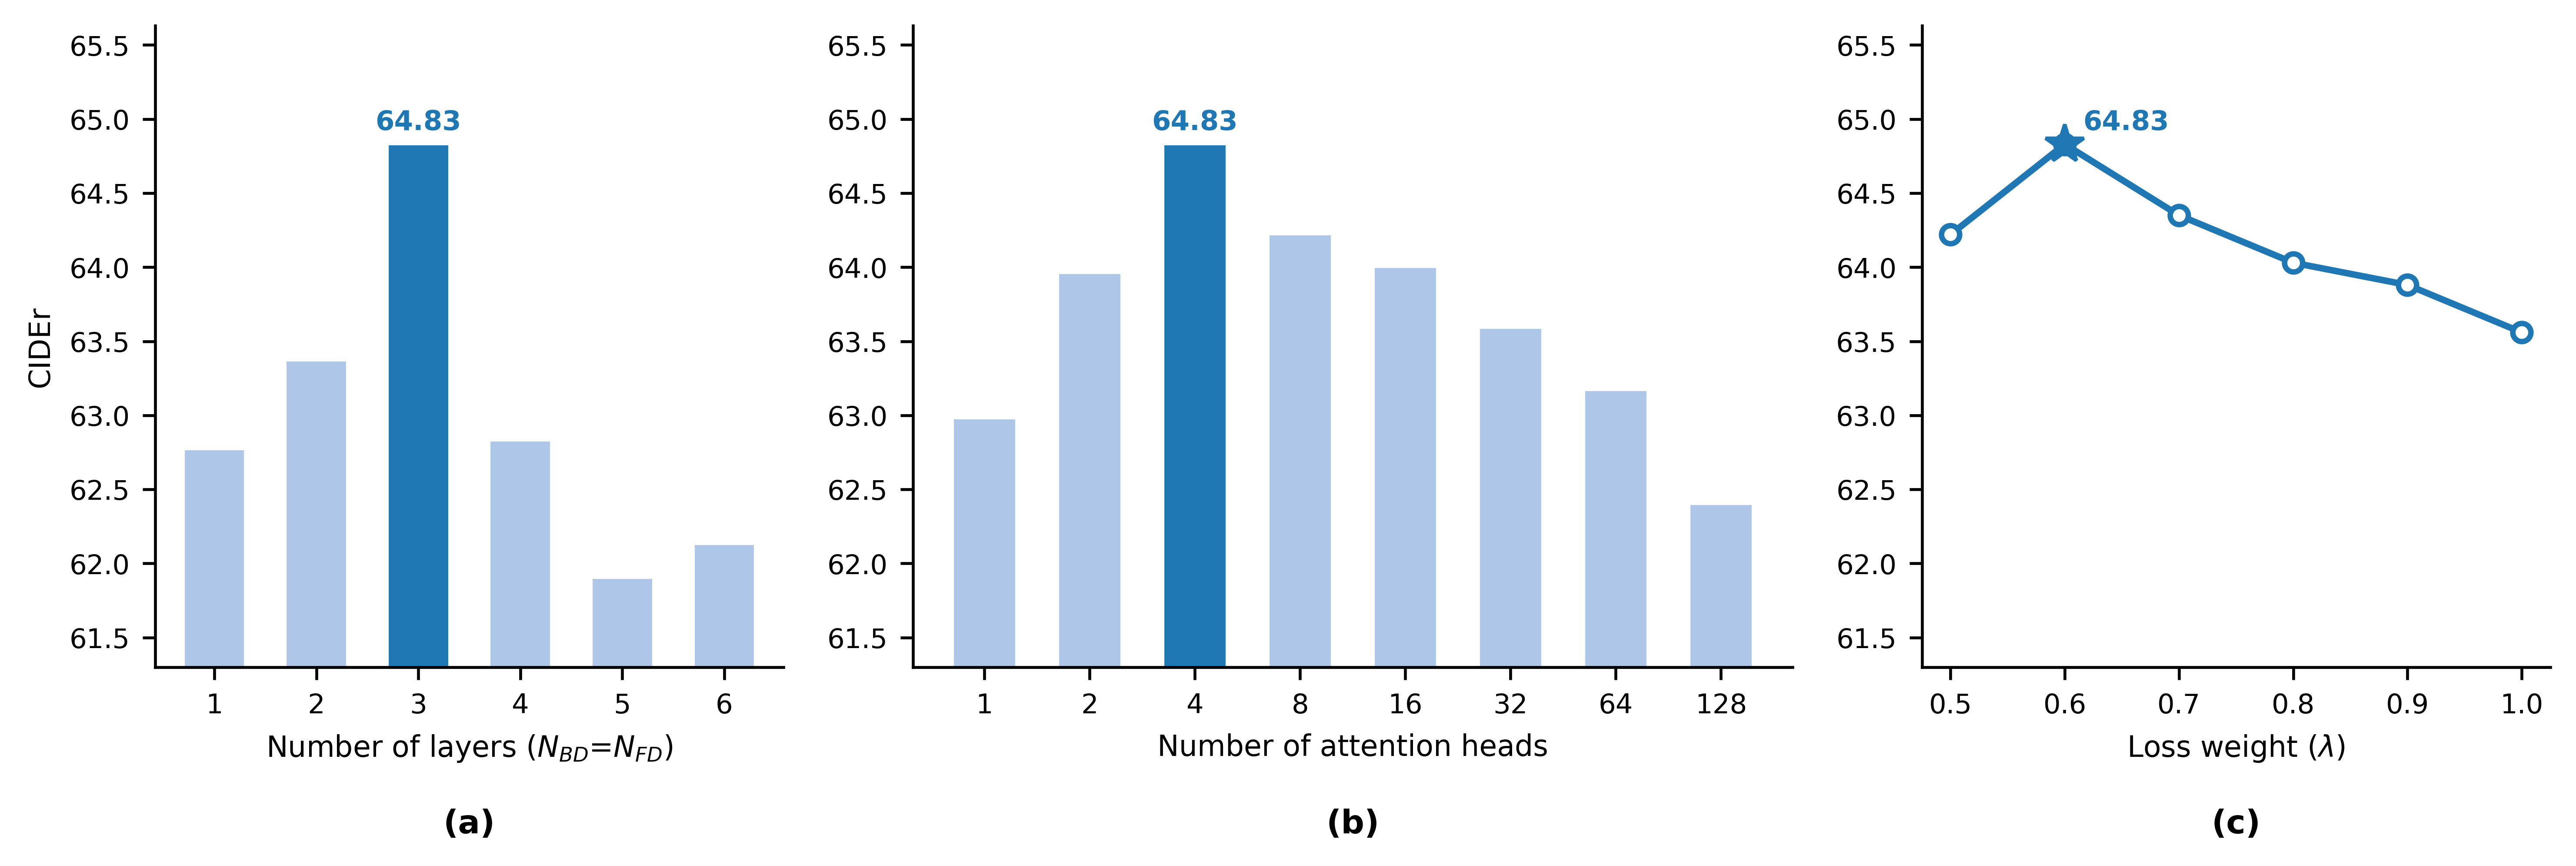
\includegraphics[width=0.85\textwidth, height=8.5in, keepaspectratio]{figures/fig06_exp_hyperparams.png}
\caption{Hyperparameter sensitivity analysis on MSR-VTT, reporting CIDEr on the test set. (a) Effect of decoder depth with $N_{BD}=N_{FD}$. (b) Effect of attention head count. (c) Effect of loss-balancing coefficient $\lambda$. Highlighted bars and the star marker denote the selected configuration.}
\label{fig:fig06_exp_hyperparams}
\end{figure*}

To analyze the sensitivity of BiDecT to key hyperparameters, all experiments in this section are conducted on MSR-VTT. Results are summarized in Fig.~\ref{fig:fig06_exp_hyperparams} and Table~\ref{tab:exp_max_gops}.

For decoder depth (see Fig.~\ref{fig:fig06_exp_hyperparams} \hyperref[fig:fig06_exp_hyperparams]{(a)}), CIDEr improves from 62.77 at $N\,\texttt{=}\,1$ to 64.83 at $N\,\texttt{=}\,3$, before declining for deeper configurations and reaching 61.90 at $N\,\texttt{=}\,5$. The improvement from $N\,\texttt{=}\,1$ to $N\,\texttt{=}\,3$ reflects the benefit of additional capacity for modeling multimodal-to-text dependencies. The decline beyond $N\,\texttt{=}\,3$ suggests that deeper architectures introduce optimization difficulty and diminishing representational returns in this setting. Three decoder layers are therefore adopted as the default configuration.

A similar sensitivity pattern is observed for the number of attention heads (see Fig.~\ref{fig:fig06_exp_hyperparams} \hyperref[fig:fig06_exp_hyperparams]{(b)}). Performance peaks at 4 heads (64.83) and gradually declines as the head count increases, reaching 62.40 at 128 heads. With $d_{\textit{model}}\,\texttt{=}\,512$, the per-head subspace dimension is $d_{\textit{model}}/h$; at 4 heads, each head operates on a 128-dimensional subspace. This configuration balances attention diversity and per-head representational capacity. As $h$ increases beyond 4, the per-head dimension becomes increasingly small, limiting each head’s ability to capture meaningful patterns. Four attention heads are therefore adopted as the default configuration.

Fig.~\ref{fig:fig06_exp_hyperparams} \hyperref[fig:fig06_exp_hyperparams]{(c)} illustrates the effect of the loss-balancing coefficient $\lambda$, which exhibits a similarly non-monotonic pattern. CIDEr peaks at $\lambda\,\texttt{=}\,0.6$ (64.83) and gradually decreases toward $\lambda\,\texttt{=}\,1$ (63.56), where the BD receives no direct supervision from its own objective and must rely solely on indirect gradients propagated through $\mathcal{L}_{\textit{FD}}$. The optimal value $\lambda\,\texttt{=}\,0.6$ ensures that the BD receives sufficient direct supervision to construct meaningful backward contextual representations $\MyLVec[1]{H}$ for conditioning the FD, and is therefore adopted as the default configuration.


Table~\ref{tab:exp_max_gops} reports the effect of the maximum number of GOPs $G$ sampled per video, with $\mathrm{KeyInt}$ fixed at 45. CIDEr increases from 63.46 at \mbox{$G\,\texttt{=}\,6$} (P25) to 64.83 at \mbox{$G\,\texttt{=}\,10$} (P75) as the model gains access to more temporal segments, before declining slightly to 64.37 at \mbox{$G\,\texttt{=}\,12$} (P90). The decline beyond $G\,\texttt{=}\,10$ suggests that GOPs beyond the 75th percentile introduce redundant content without additional discriminative benefit. Moreover, total inference time increases only modestly across all configurations, from 443.56 seconds at \mbox{$G\,\texttt{=}\,6$} to 451.19 seconds at \mbox{$G\,\texttt{=}\,12$}, confirming that the linear $\mathcal{O}(G)$ scaling of the encoder-free architecture translates to low computational overhead. The 75th percentile is therefore adopted as the default GOP count across all datasets.

\begin{table}[!t]
\caption{Effect of the maximum number of GOPs per video ($G$) on MSR-VTT. P$x$ denotes the $x$-th percentile of the GOP-count distribution in the MSR-VTT training set. Time (s) denotes total inference time on the test set, measured on a NVIDIA Tesla P100 GPU. $\dagger$ denotes the default configuration.}
\label{tab:exp_max_gops}
\centering
\begin{tabular}{l c cccc}
\hline\hline
 & & \multicolumn{4}{c}{\textbf{MSR-VTT}} \\
\cline{3-6}
\textbf{Max GOPs} & \textbf{Time (s)} & \textbf{B4} & \textbf{M} & \textbf{R} & \textbf{C} \\
\hline
6 (P25) & 443.56 & 48.37 & 31.18 & 65.22 & 63.46 \\
8 (P50) & 445.27 & 48.10 & 31.25 & 64.97 & 64.06 \\
$\mathbf{10}$ \textbf{(P75)}$^\dagger$ & \textbf{448.43} & \textbf{49.23} & \textbf{31.73} & \textbf{65.87} & \textbf{64.83} \\
12 (P90) & 451.19 & 48.76 & 31.45 & 65.50 & 64.37 \\
\hline\hline
\end{tabular}
\end{table}

% Table 7 
% Effect of the maximum number of GOPs per video (G) on MSR-VTT, with KeyInt fixed at 45. Px denotes the x-th percentile of the GOP-count distribution in the MSR-VTT training set. Time (s) denotes total inference time on the test set, measured on a single NVIDIA Tesla P100 GPU. † indicates the default BiDecT configuration.
% Max GOPs	Time (s)	MSR-VTT
% 		B4	M	R	C
% 6 (P25)	443.56	48.37	31.18	65.22	63.46
% 8 (P50)	445.27	48.10	31.25	64.97	64.06
% 10 (P75)†	448.43	49.23	31.73	65.87	64.83
% 12 (P90)	451.19	48.76	31.45	65.50	64.37




\subsection{Ablation Study}
\label{subsec:subsec_56_ablation}
To assess the contribution of each design component, all experiments in this section are conducted on MSR-VTT.

\subsubsection{Bidirectional Decoding}
\label{subsubsec:subsubsec_561_exp_decoding}
Fig.~\ref{fig:fig07_exp_decoding_comparison} compares BiDecT (FD+BD) against a unidirectional baseline (FD-only) in which the FD conditions solely on the multimodal representation $\MyRVec[1]{E}$ without access to backward context. Bidirectional decoding yields consistent improvements across all four metrics: CIDEr improves from 60.31 to 64.83 (+4.52), with additional gains of +2.53 ROUGE-L, +1.75 BLEU@4, and +1.00 METEOR. Notably, CIDEr and ROUGE-L, which capture sentence-level consensus, exhibit larger improvements than BLEU@4 and METEOR, which focus on local lexical overlap. This suggests that $\MyLVec[1]{H}$ provides a global preview of caption structure, enabling the FD to plan more coherent outputs rather than merely improving token-level precision. The importance of maintaining the integrity of this backward context through the pseudo reverse caption strategy is examined in the next section.

\begin{figure}[!t]
\centering
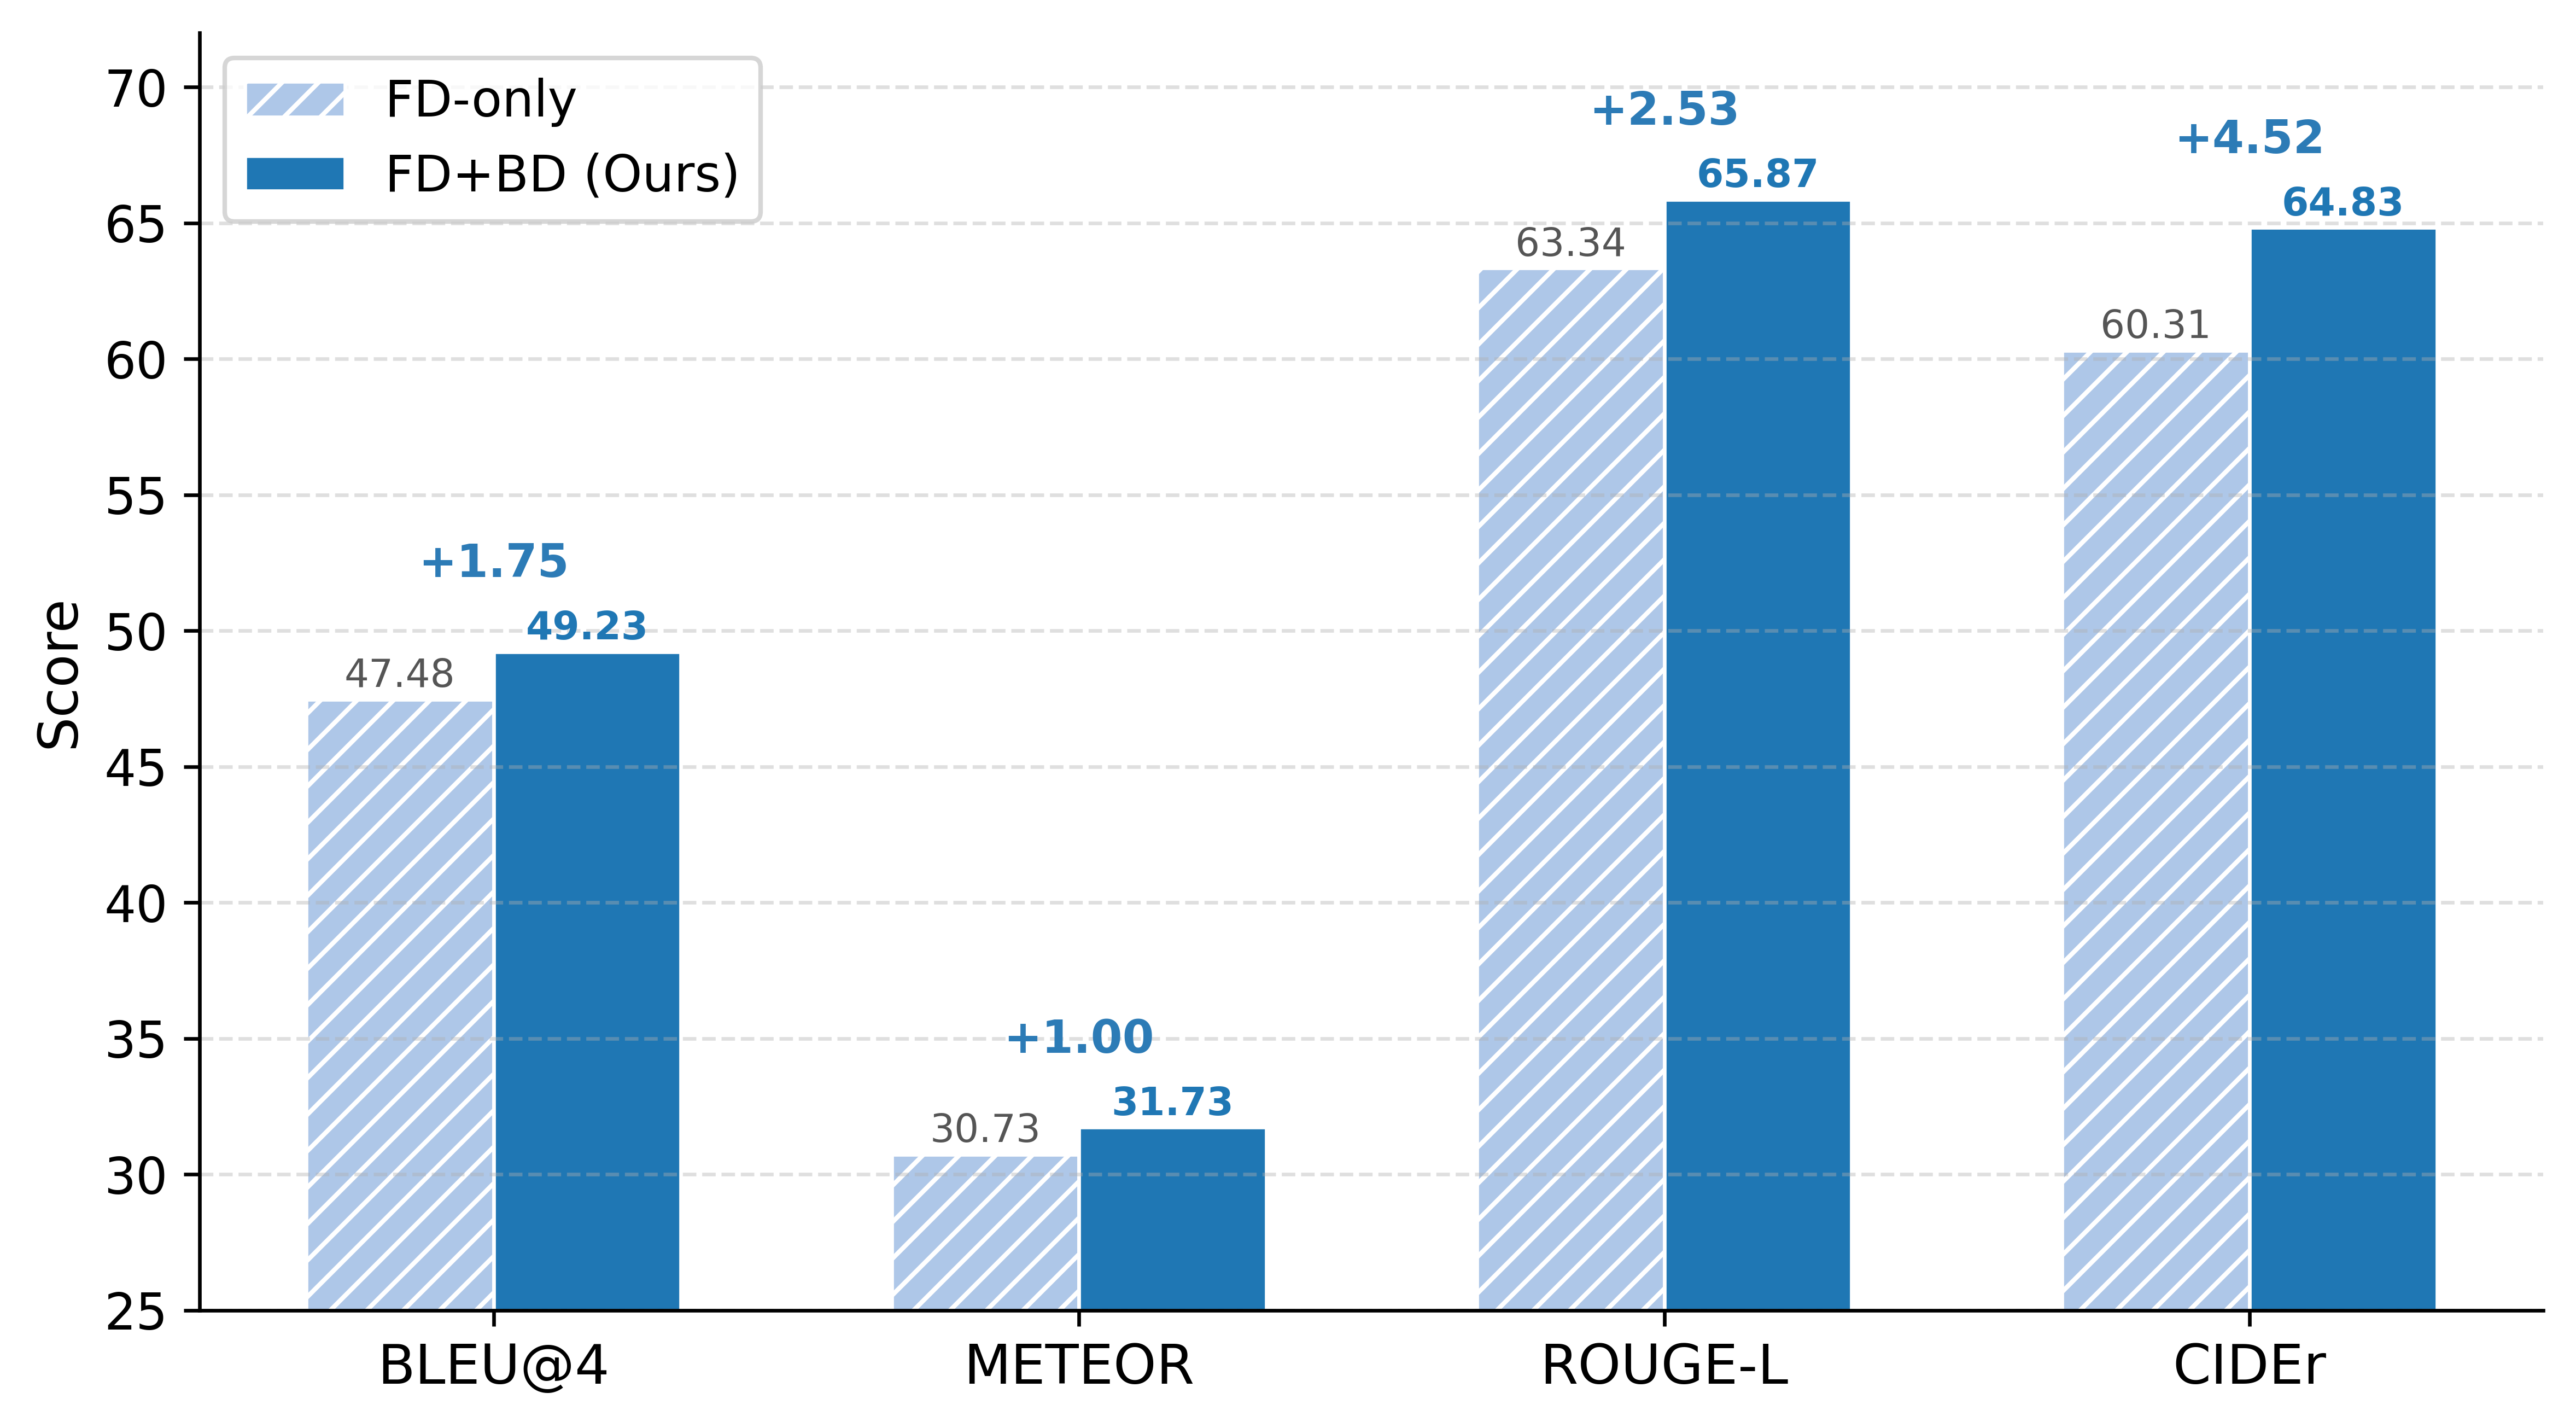
\includegraphics[width=0.85\columnwidth]{figures/fig07_exp_decoding_comparison.png}
\caption{Effect of bidirectional decoding on the MSR-VTT test set. FD-only denotes the unidirectional baseline, while FD+BD denotes BiDecT. Delta values above each bar pair indicate the absolute improvement from FD-only to FD+BD.}
\label{fig:fig07_exp_decoding_comparison}
\end{figure}


\subsubsection{Pseudo Reverse Caption}
\label{subsubsec:subsubsec_562_exp_prc}
As discussed in Section~\ref{subsec:subsec_46_optim}, training bidirectional decoders without the pseudo reverse caption (PRC) strategy introduces information leakage, where the FD exploits token-level correspondence between $\MyLVec[1]{H}$ and the target caption instead of learning to generate from multimodal input. Fig.~\ref{fig:fig08_exp_prc_analysis} provides direct empirical evidence. When the BD is supervised using the exact reversal of the forward caption (Fig.~\ref{fig:fig08_exp_prc_analysis} \hyperref[fig:fig08_exp_prc_analysis]{(a)}), $\mathcal{L}_{\textit{FD}}$ drops sharply to 0.28 by epoch 16, while $\mathcal{L}_{\textit{BD}}$ converges only to 2.463, a gap of approximately 8.8$\times$. In contrast, when applying PRC (Fig.~\ref{fig:fig08_exp_prc_analysis} \hyperref[fig:fig08_exp_prc_analysis]{(b)}), both losses converge to comparable values (2.107 and 2.137), confirming that both decoders face similarly challenging generation tasks without a trivial shortcut.

Fig.~\ref{fig:fig08_exp_prc_analysis} \hyperref[fig:fig08_exp_prc_analysis]{(c)} reports the test CIDEr scores of both decoders under each condition. Without PRC, the FD achieves only 58.36, while the BD reaches 60.53. This inverted ranking directly reflects the leakage: the FD merely copies from $\MyLVec[1]{H}$ rather than learning to generate from multimodal input. This shortcut collapses at inference time: without ground-truth access, the BD produces $\MyLVec[1]{H}$ that differs from what the FD was trained to exploit, causing the FD score of 58.36 to fall below even the FD-only baseline of 60.31 (dashed line). The BD itself achieves only 60.53, marginally exceeding the baseline, indicating that exact-reversal training also constrains its ability to learn generalizable representations.

With PRC, the expected ranking is restored: the FD achieves 64.83, surpassing the BD score of 63.04. This confirms that the FD now properly leverages backward contextual information for improved generation. The BD itself also improves substantially from 60.53 to 63.04 (+2.51), suggesting that pseudo-pairing acts as implicit data augmentation by exposing the BD to diverse reverse captions for the same video. The PRC strategy is therefore essential for bidirectional decoding to realize its intended benefit.

\begin{figure*}[!t]
\centering
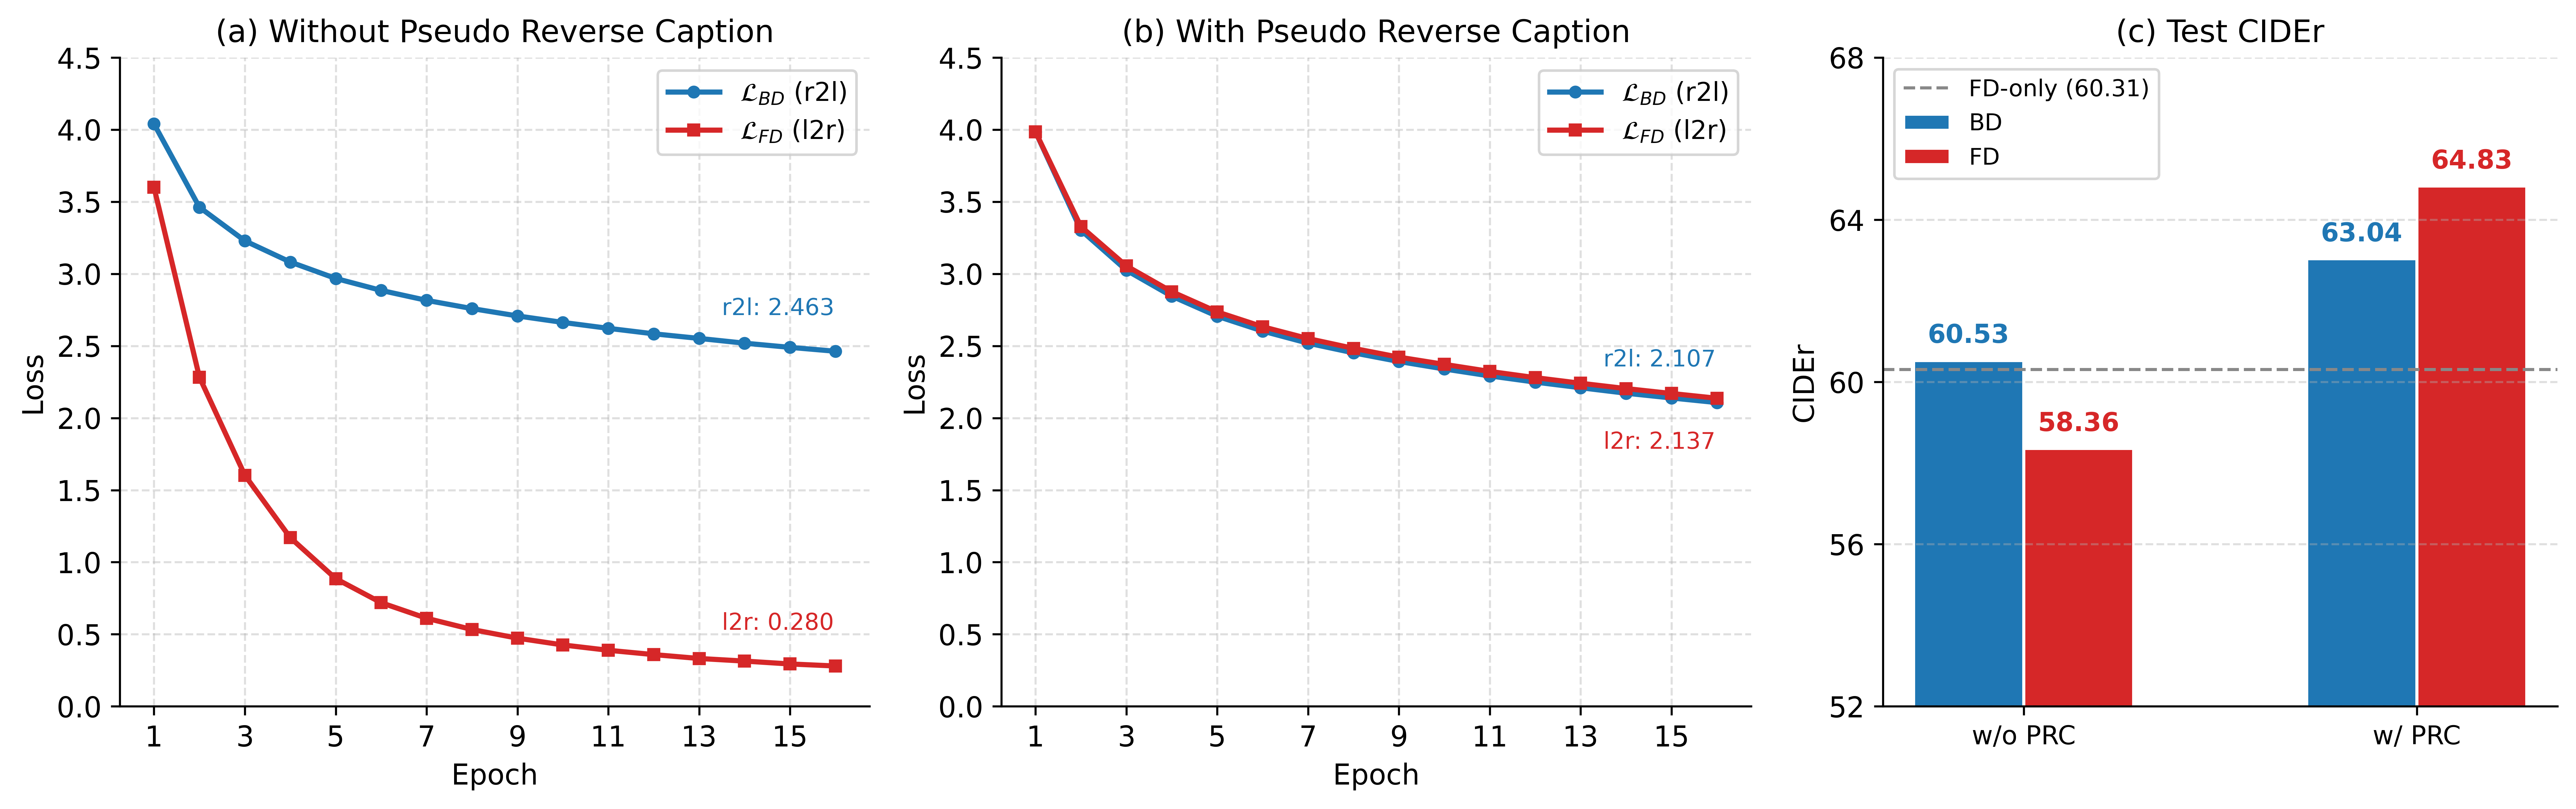
\includegraphics[width=0.85\textwidth, height=8.5in, keepaspectratio]{figures/fig08_exp_prc_analysis.png}
\caption{Effect of the pseudo reverse caption (PRC) strategy on MSR-VTT. (a) and (b) show training loss curves for $\mathcal{L}_{BD}$ and $\mathcal{L}_{FD}$ over 16 epochs without and with PRC, respectively. (c) compares the test CIDEr scores of the BD and FD under each condition. The dashed line indicates the FD-only baseline.}
\label{fig:fig08_exp_prc_analysis}
\end{figure*}


\subsubsection{Input Modalities}
\label{subsubsec:subsubsec_563_exp_input}
Table~\ref{tab:exp_input_modality} summarizes ablation results on input modalities and embedding design choices.

\begin{table*}[!t]
\caption{Ablation study on input modalities and embedding module design, evaluated on the MSR-VTT test set. App, Sem, and Mot denote appearance, semantic, and motion features, respectively. Type Emb indicates whether modality-specific type embeddings are applied. Ind.\ Emb.\ indicates whether the backward and forward decoders use independent (\checkmark) or shared ($-$) embedding modules.}
\label{tab:exp_input_modality}
\centering
\begin{tabular}{ccccc cccc}
\hline\hline
 & & & & & \multicolumn{4}{c}{\textbf{MSR-VTT}} \\
\cline{6-9}
\textbf{App} & \textbf{Sem} & \textbf{Mot} & \textbf{Type Emb} & \textbf{Ind. Emb.} & \textbf{B4} & \textbf{M} & \textbf{R} & \textbf{C} \\
\hline
\checkmark & $-$ & $-$ & $-$ & \checkmark & 46.86 & 30.98 & 64.55 & 61.79 \\
$-$ & \checkmark & $-$ & $-$ & \checkmark & 45.39 & 30.42 & 63.62 & 60.32 \\
$-$ & $-$ & \checkmark & $-$ & \checkmark & 40.10 & 28.24 & 59.60 & 51.02 \\
\checkmark & \checkmark & $-$ & \checkmark & \checkmark & 48.35 & 31.56 & 65.07 & 63.32 \\
\checkmark & $-$ & \checkmark & \checkmark & \checkmark & 47.62 & 31.18 & 64.74 & 62.34 \\
$-$ & \checkmark & \checkmark & \checkmark & \checkmark & 47.11 & 30.92 & 64.27 & 61.17 \\
\checkmark & \checkmark & \checkmark & $-$ & \checkmark & 47.27 & 30.82 & 64.50 & 61.18 \\
\checkmark & \checkmark & \checkmark & \checkmark & $-$ & 48.74 & 31.45 & 65.55 & 62.53 \\
\checkmark & \checkmark & \checkmark & \checkmark & \checkmark & \textbf{49.23} & \textbf{31.73} & \textbf{65.87} & \textbf{64.83} \\
\hline\hline
\end{tabular}
\end{table*}

% Table 8 
% Ablation study on input modalities and embedding module design, evaluated on the MSR-VTT test set. App, Sem, and Mot denote appearance, semantic, and motion features, respectively. Type Emb indicates whether modality-specific type embeddings are applied. Ind. Emb. indicates whether the backward and forward decoders use independent (✓) or shared (−) embedding modules.
% App	Sem	Mot	Type Emb	Ind. Emb.	MSR-VTT
% 					B4	M	R	C
% ✓	−	−	−	✓	46.86	30.98	64.55	61.79
% −	✓	−	−	✓	45.39	30.42	63.62	60.32
% −	−	✓	−	✓	40.10	28.24	59.60	51.02
% ✓	✓	−	✓	✓	48.35	31.56	65.07	63.32
% ✓	−	✓	✓	✓	47.62	31.18	64.74	62.34
% −	✓	✓	✓	✓	47.11	30.92	64.27	61.17
% ✓	✓	✓	−	✓	47.27	30.82	64.50	61.18
% ✓	✓	✓	✓	−	48.74	31.45	65.55	62.53
% ✓	✓	✓	✓	✓	49.23	31.73	65.87	64.83

Among single-modality settings, appearance features achieve the highest CIDEr (61.79), followed by semantic features (60.32) and motion features (51.02). Both appearance and semantic features are derived from BLIP-2, whereas motion features are extracted from MViTv2. The substantial gap between VLM-derived features and motion features suggests that representations capturing both visual content and language alignment provide a stronger foundation for caption generation. All two-modality combinations outperform their constituent single-modality results, with appearance + semantic, appearance + motion, and semantic + motion achieving 63.32, 62.34, and 61.17 CIDEr, respectively. The full three-modality configuration achieves the best performance (64.83), confirming that all three modalities provide complementary information.

The results also reveal the importance of the embedding module design introduced in Section~\ref{subsec:subsec_43_feat_emb}. Without modality-specific type embeddings, the three-modality configuration achieves only 61.18 CIDEr, lower than appearance features alone (61.79). This indicates that without type embeddings, the decoder cannot distinguish tokens from different modalities, causing features to interfere rather than complement one another. Furthermore, using independent embedding modules for the BD and FD (64.83) outperforms a shared module (62.53) by 2.30 points. Because the two decoders operate on opposite caption directions, a shared module must optimize for conflicting objectives, creating parameter conflict. Independent modules allow each decoder to learn its own modality-specific transformations, while type embeddings preserve modality identity within each stream.


\subsubsection{Layer Normalization Strategy}
\label{subsubsec:subsubsec_564_exp_ln}
To evaluate the impact of normalization placement on training stability and final performance, we compare the three strategies: Post-LN, Pre-LN, and Peri-LN. Results are summarized in Fig.~\ref{fig:fig09_exp_ln_comparison}.

\begin{figure}[!t]
\centering
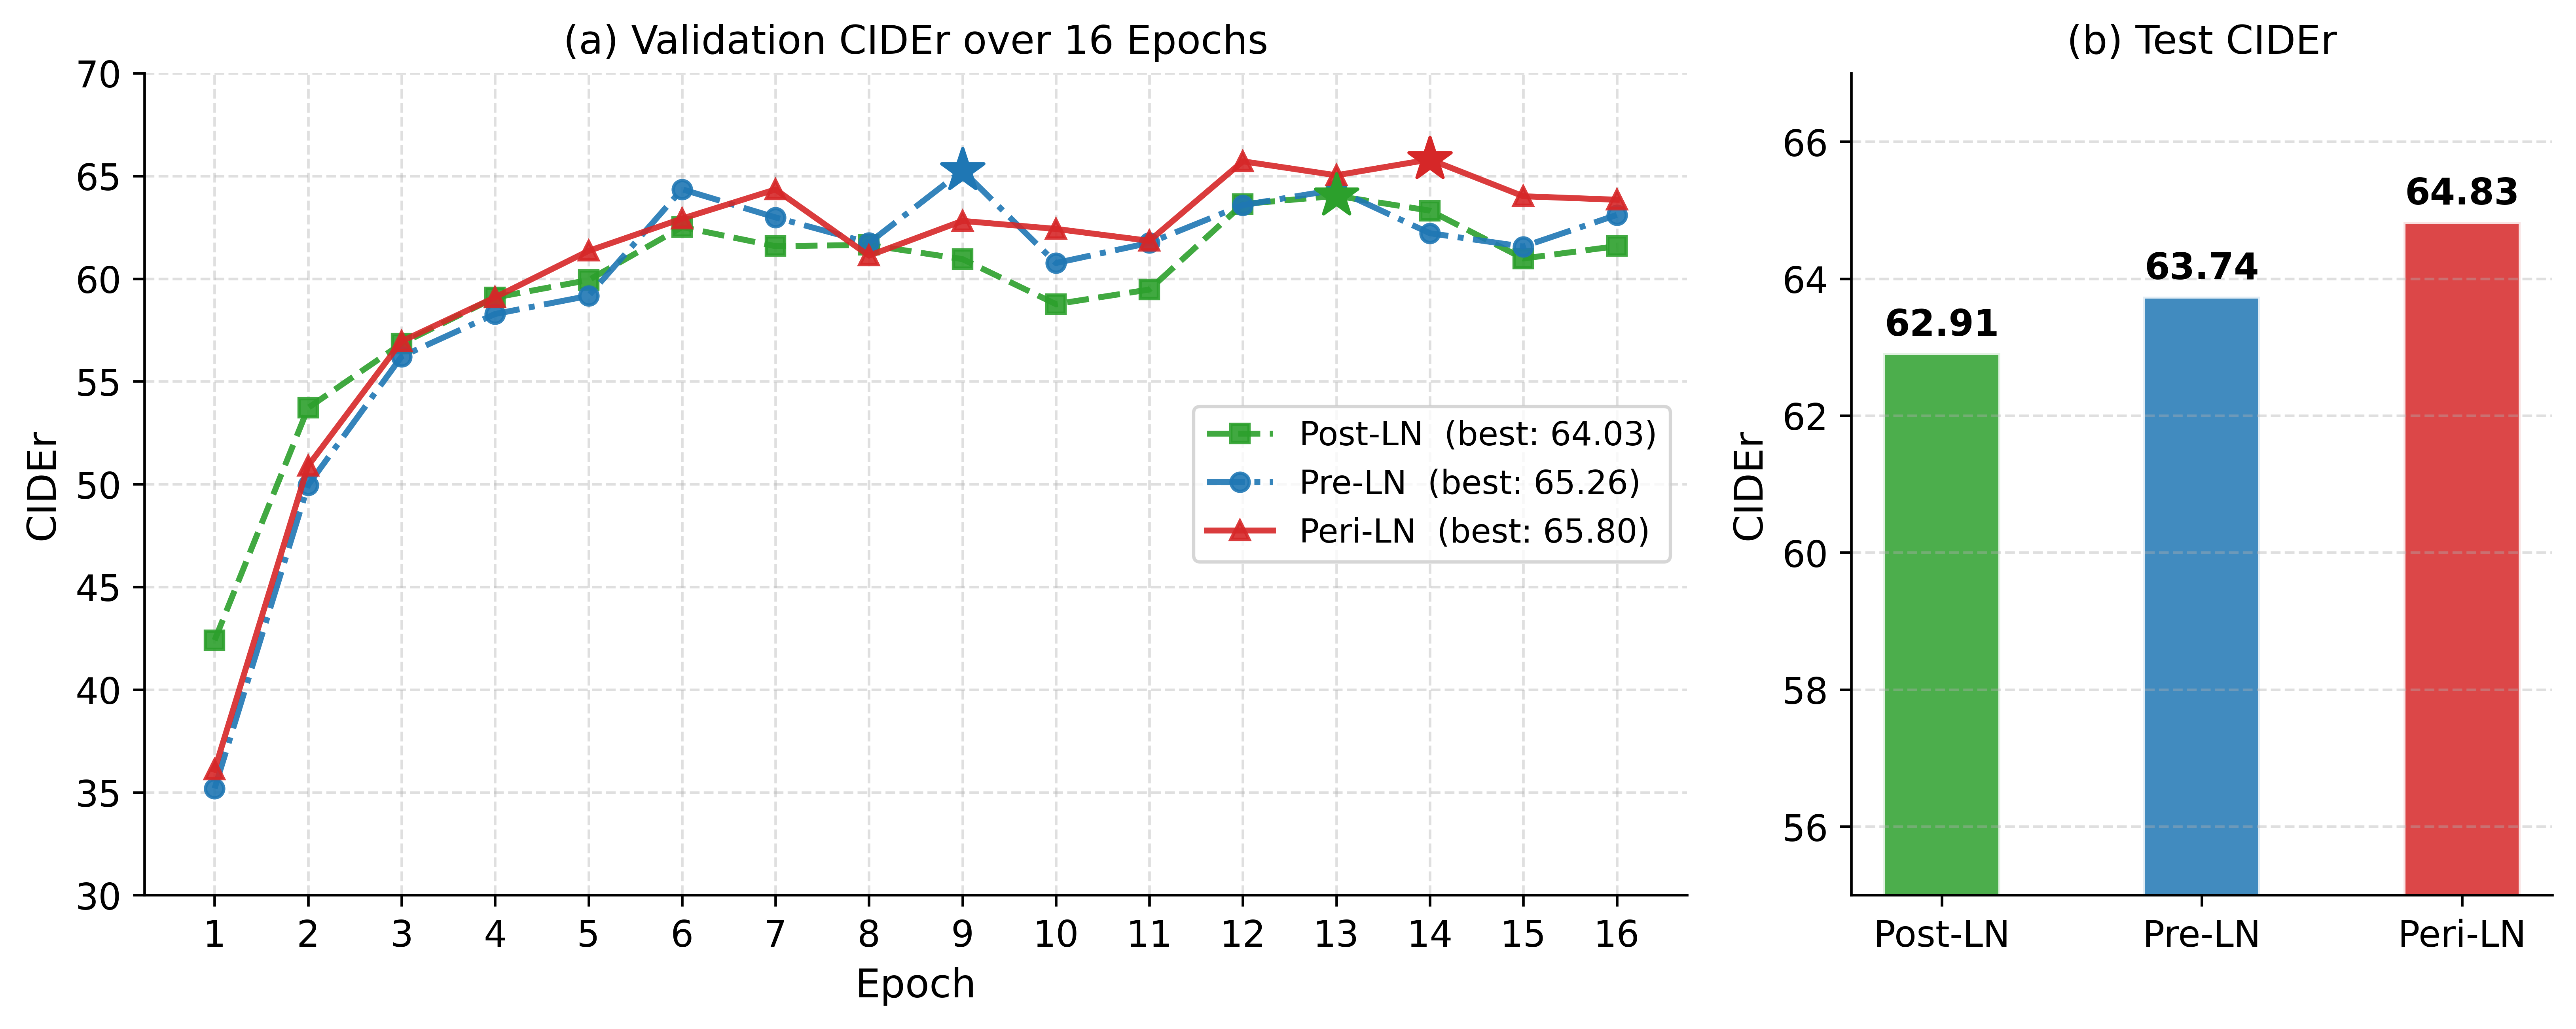
\includegraphics[width=0.99\columnwidth]{figures/fig09_exp_ln_comparison.png}
\caption{Comparison of layer normalization strategies on MSR-VTT. (a) Validation CIDEr over 16 training epochs; star markers denote the best epoch for each strategy. (b) Test CIDEr of the checkpoint selected at the best validation epoch.}
\label{fig:fig09_exp_ln_comparison}
\end{figure}

% Fig.~\ref{fig:fig09_exp_ln_comparison} \hyperref[fig:fig09_exp_ln_comparison]{(?)}
As shown in Fig.~\ref{fig:fig09_exp_ln_comparison} \hyperref[fig:fig09_exp_ln_comparison]{(b)}, Peri-LN achieves the highest test CIDEr (64.83), outperforming Pre-LN (63.74) and Post-LN (62.91) by 1.09 and 1.92 points, respectively. The validation curves in Fig.~\ref{fig:fig09_exp_ln_comparison} \hyperref[fig:fig09_exp_ln_comparison]{(a)} provide additional insight into training dynamics. Post-LN exhibits the slowest convergence and highest variance across epochs. Pre-LN converges more stably in early epochs but exhibits variance accumulation in later stages, achieving a best validation CIDEr of 65.26 at epoch 13. Peri-LN maintains the most stable validation trajectory, reaching 65.80 at epoch 14, higher than both Post-LN (64.03) and Pre-LN (65.26).

This ranking is consistent with the theoretical analysis. Post-LN can weaken gradient flow by requiring gradients to pass through the normalization layer, while Pre-LN improves propagation but normalizes only the module input, allowing hidden state variance to grow across layers. Peri-LN addresses both limitations by normalizing both the module input and output. These properties are particularly important in BiDecT, where gradients from $\mathcal{L}_{\textit{FD}}$ propagate not only through the FD but also back through the BD, since the FD conditions on $\MyLVec[1]{H}$ produced by the BD. This creates a longer gradient pathway than in unidirectional decoders, making tight control over hidden state magnitudes at every sub-layer essential for stable joint optimization. Peri-LN provides this control, making it well suited to the bidirectional architecture of BiDecT.


\subsection{Case Study}
\label{subsec:subsec_57_case_study}
To complement the quantitative evaluation, Fig.~\ref{fig:fig10_case_study} presents qualitative examples from all three benchmark datasets. We select four success cases and one failure case to illustrate how the generated captions reflect the proposed design choices and to identify remaining limitations.

\begin{figure*}[!t]
\centering
\includegraphics[width=0.85\textwidth, height=8.5in, keepaspectratio]{figures/fig10_case_study_2.png}
\caption{Qualitative examples of captions generated by BiDecT on MSVD, MSR-VTT, and VATEX. For each video, representative frames are shown alongside two ground-truth (GT) captions and the model prediction (Pred). {\textcolor[HTML]{00B050}{\textbf{Bold green text}}} denotes correctly predicted key terms; {\textcolor[HTML]{FF0000}{\textbf{bold red text}}} denotes hallucinated content; {\textcolor[HTML]{ED7D31}{\MyULine{underlined orange text}}} in ground-truth captions marks important details not captured by the prediction.}
\label{fig:fig10_case_study}
\end{figure*}

Examples (a), (b), and (c) demonstrate accurate identification of objects, attributes, and actions. For the MSVD cooking scene (a), BiDecT generates ``\textit{a girl slowly adds milk to a bowl of eggs}," capturing both the scene objects and the manner of the action. For the MSR-VTT makeup tutorial (c), it produces ``\textit{a woman is applying red lipstick}," identifying the product and its specific color attribute. This descriptive specificity is consistent with the multimodal ablation results: appearance features capture visual entities and attributes, while VLM-derived semantic features provide higher-level activity context that supports precise descriptions. In example (b), the prediction ``\textit{three boys are performing a dance}" correctly identifies both the number of participants and their activity, although the audience context present in the reference captions is omitted. This partial omission is consistent with the known tendency of captioning models to focus on primary foreground actions rather than background context.

Example (d) demonstrates temporal understanding: BiDecT generates ``\textit{a man blows up a blue balloon and then twists it to make a shape}," capturing a multi-step action sequence in chronological order. This temporal awareness reflects two complementary design choices: the GOP-based sampling strategy, which distributes the input across distinct temporal segments to capture evolving scene content, and the global backward context $\MyLVec[1]{H}$, which enables the FD to plan a coherent sequential description before committing to individual tokens.

Example (e) illustrates a remaining limitation. The video shows a woman yawning in her room, but BiDecT generates ``\textit{a girl is sitting in a room and singing loudly}," accurately identifying the setting while hallucinating the core action. The visual similarity between yawning and singing, both involving a wide-open mouth and similar facial motion, misleads the model into substituting the ambiguous action with a more statistically frequent alternative. Notably, one of the ten human annotators for the same video also described the action as ``\textit{singing out loud with her mouth wide open}," confirming that the ambiguity is genuinely present in the visual content. This case indicates that while the current multimodal features are effective for object identification and temporal pattern recognition, they remain insufficient for discriminating between visually similar fine-grained actions. Addressing this limitation likely requires either finer-grained temporal features at the sub-GOP level or complementary audio-visual signals.
